\chapter{Improvement of the rejection of the internal Thallium-$208$ background}
\label{ch:timediff}

At the end of September 2018, the Selenium-$82$ source foils were installed on the demonstrator.
At this time, the internal \Tl\ and \Bi\ activities had already been measured by the BiPo detector.
In this chapter, we focus on rejection techniques optimised to have a high efficiency on internal \Tl\ events.



\section{Motivations for this study}

We discussed in chapter~\ref{ch:sensitivity} about the specified levels of contamination inside the source foils.
These levels are embeded by the internal \Bi\ and \Tl\ activities, given in Tab.~\ref{tab:real_target_act}.
These specifications aimed at reaching the targeted \Se\ half-life limit of $\sim1\times10^{26}$~year for a $500$ kg/y exposure.
In the same table are also given the activities measured by the BiPo detector, after the sources production.
These measurements reveal a \Tl\ contamination, about $30$ times higher than expected.
As concluded in the previous chapter, this contamination impacts the sensitivity on the $\zeronu$ decay of the final detector, decreasing it.

In this section, we work to describe the specificities of Thallium-$208$ internal background.
We will see what the methods of rejecting this background already exist.
We will also detail the basic principle of a new method we have put in place, to meet the needs of rejections of Thallium, following the measurements of BiPo.

\subsection{The internal \Tl\ background}

Trace quantities of naturally-occurring radioactive isotopes inside the source foils can occasionally produce two-electron events, and thus can mimic $\beta\beta$-decay events.
The \Tl, a progeny of \U, is one of the largest contribution to the internal background.
In fact, two electrons can be produced via $\beta$-decay followed by a M\o{}ller scattering, $\beta$-decay to an excited state with the subsequent internal conversion, or due to Compton scattering of the de-excitation photon (Fig.~\ref{fig:internal_contamination}).
\begin{figure}
  \centering
  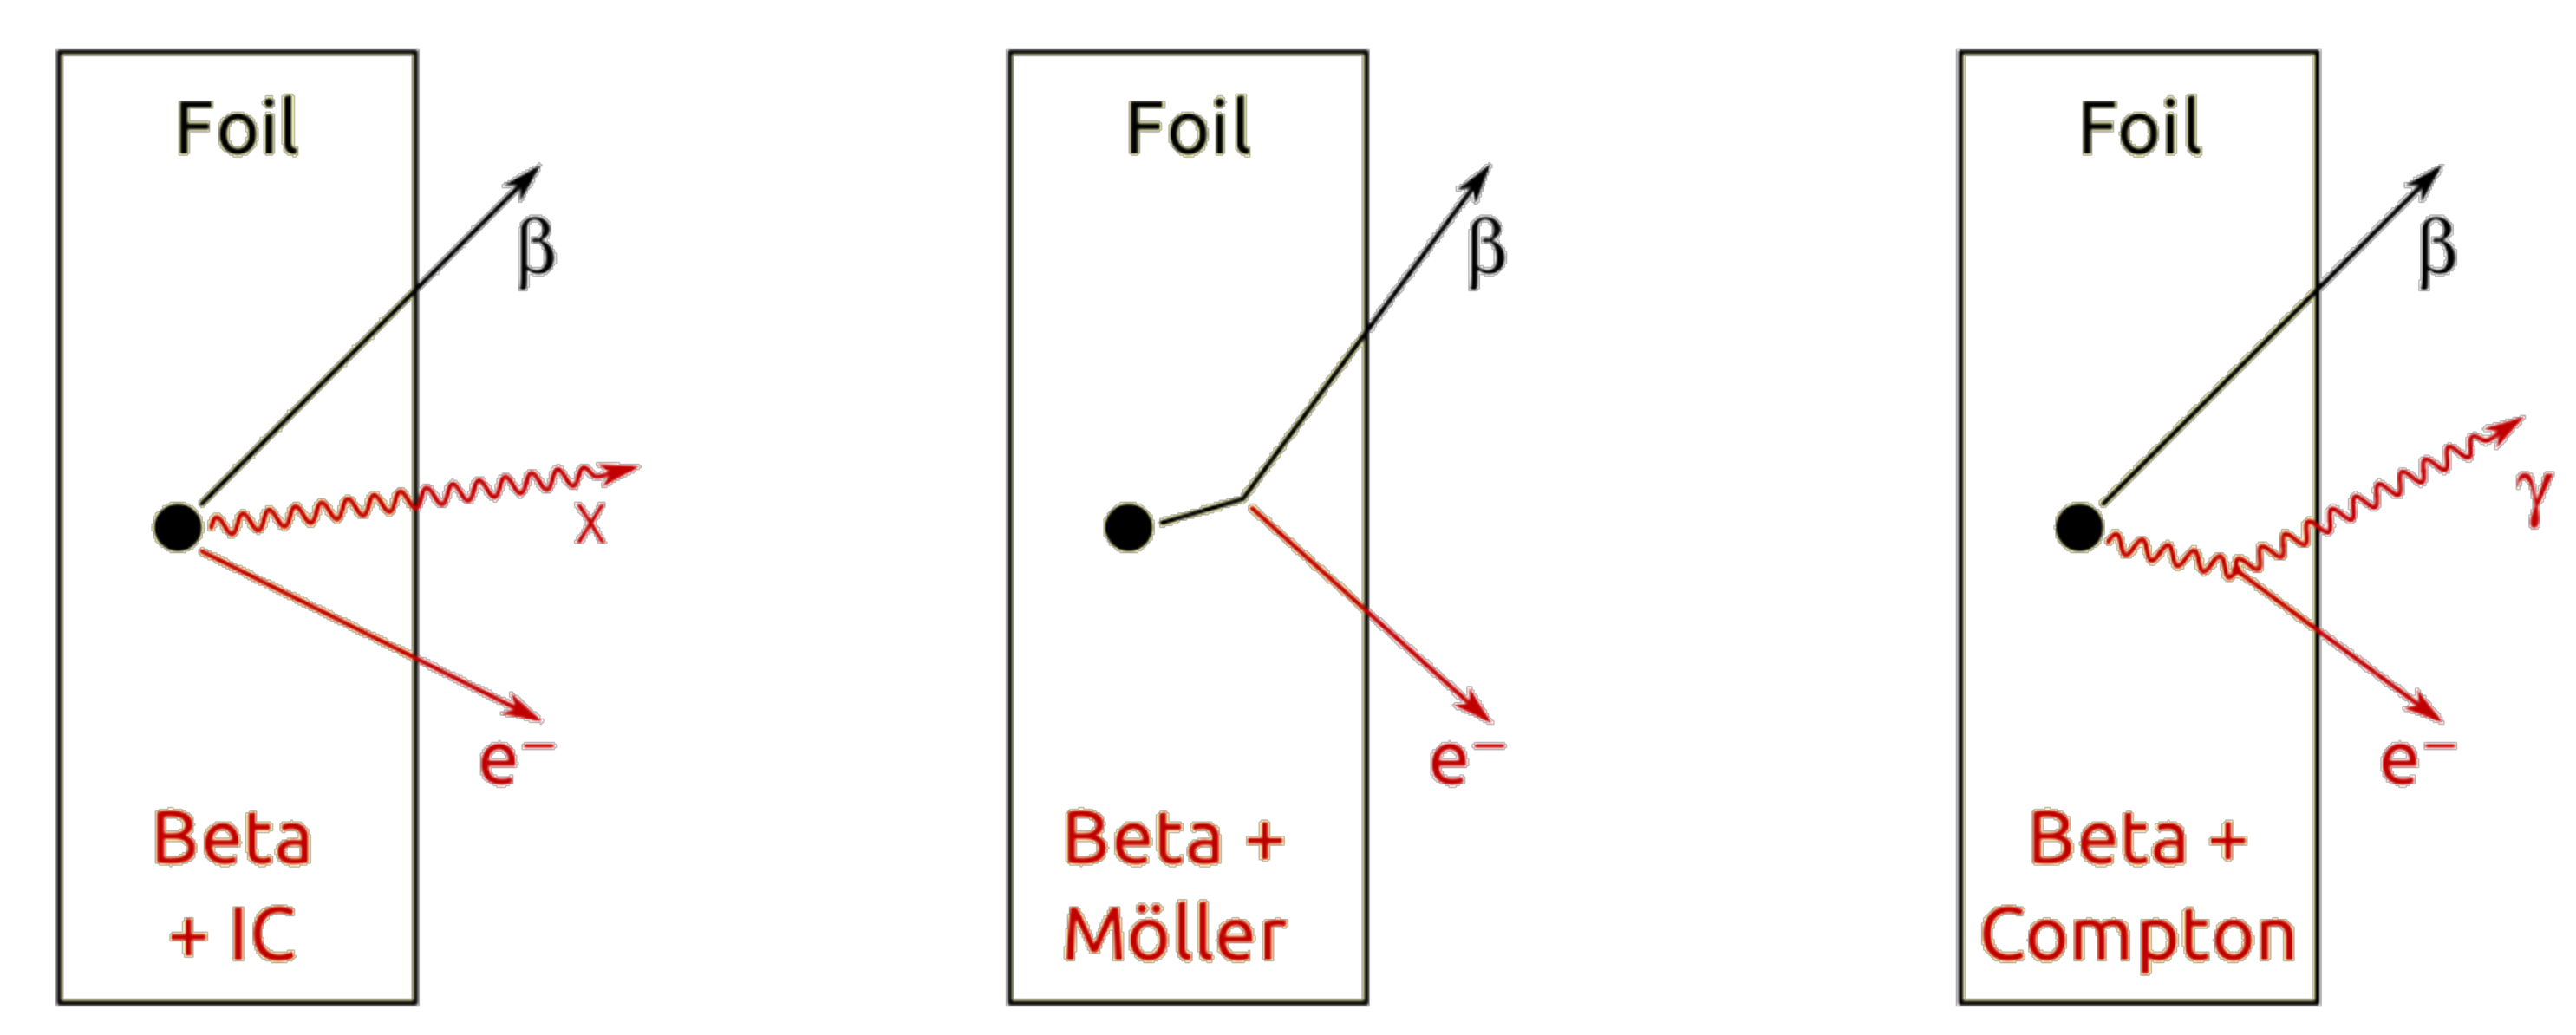
\includegraphics[width=10cm]{timedifference/fig_timediff/internal_contamination.pdf}
  \caption{(a) $\beta$ decay + internal convertion: \Tl\ nucleus performs a $\beta$ decay, then an electron is emitted after internal conversion of photon
    (b) $\beta$ decay + M\o{}ller:
    (c) $\beta$ decay + Compton diffusion: \Tl\ nucleus $\beta$ decays to an exited state, then the photon perfoms a Compton diffusion.
 \label{fig:internal_contamination}}
\end{figure}
%% The ultimate internal background for $\zeronu$ experiments is the $\twonu$ decay of the studied isotope.
%% When present in the source foils, \Tl\ and \Bi\ can mimic the $\zeronu$ signal by different processes (see Fig.~\ref{fig:internal_contamination}).

\subsection{Rejection of the \Tl\ background}
We present a simplified disintegration scheme of \Tl\ in Fig.~\ref{fig:Tl_scheme}.
\begin{figure}
  \centering
  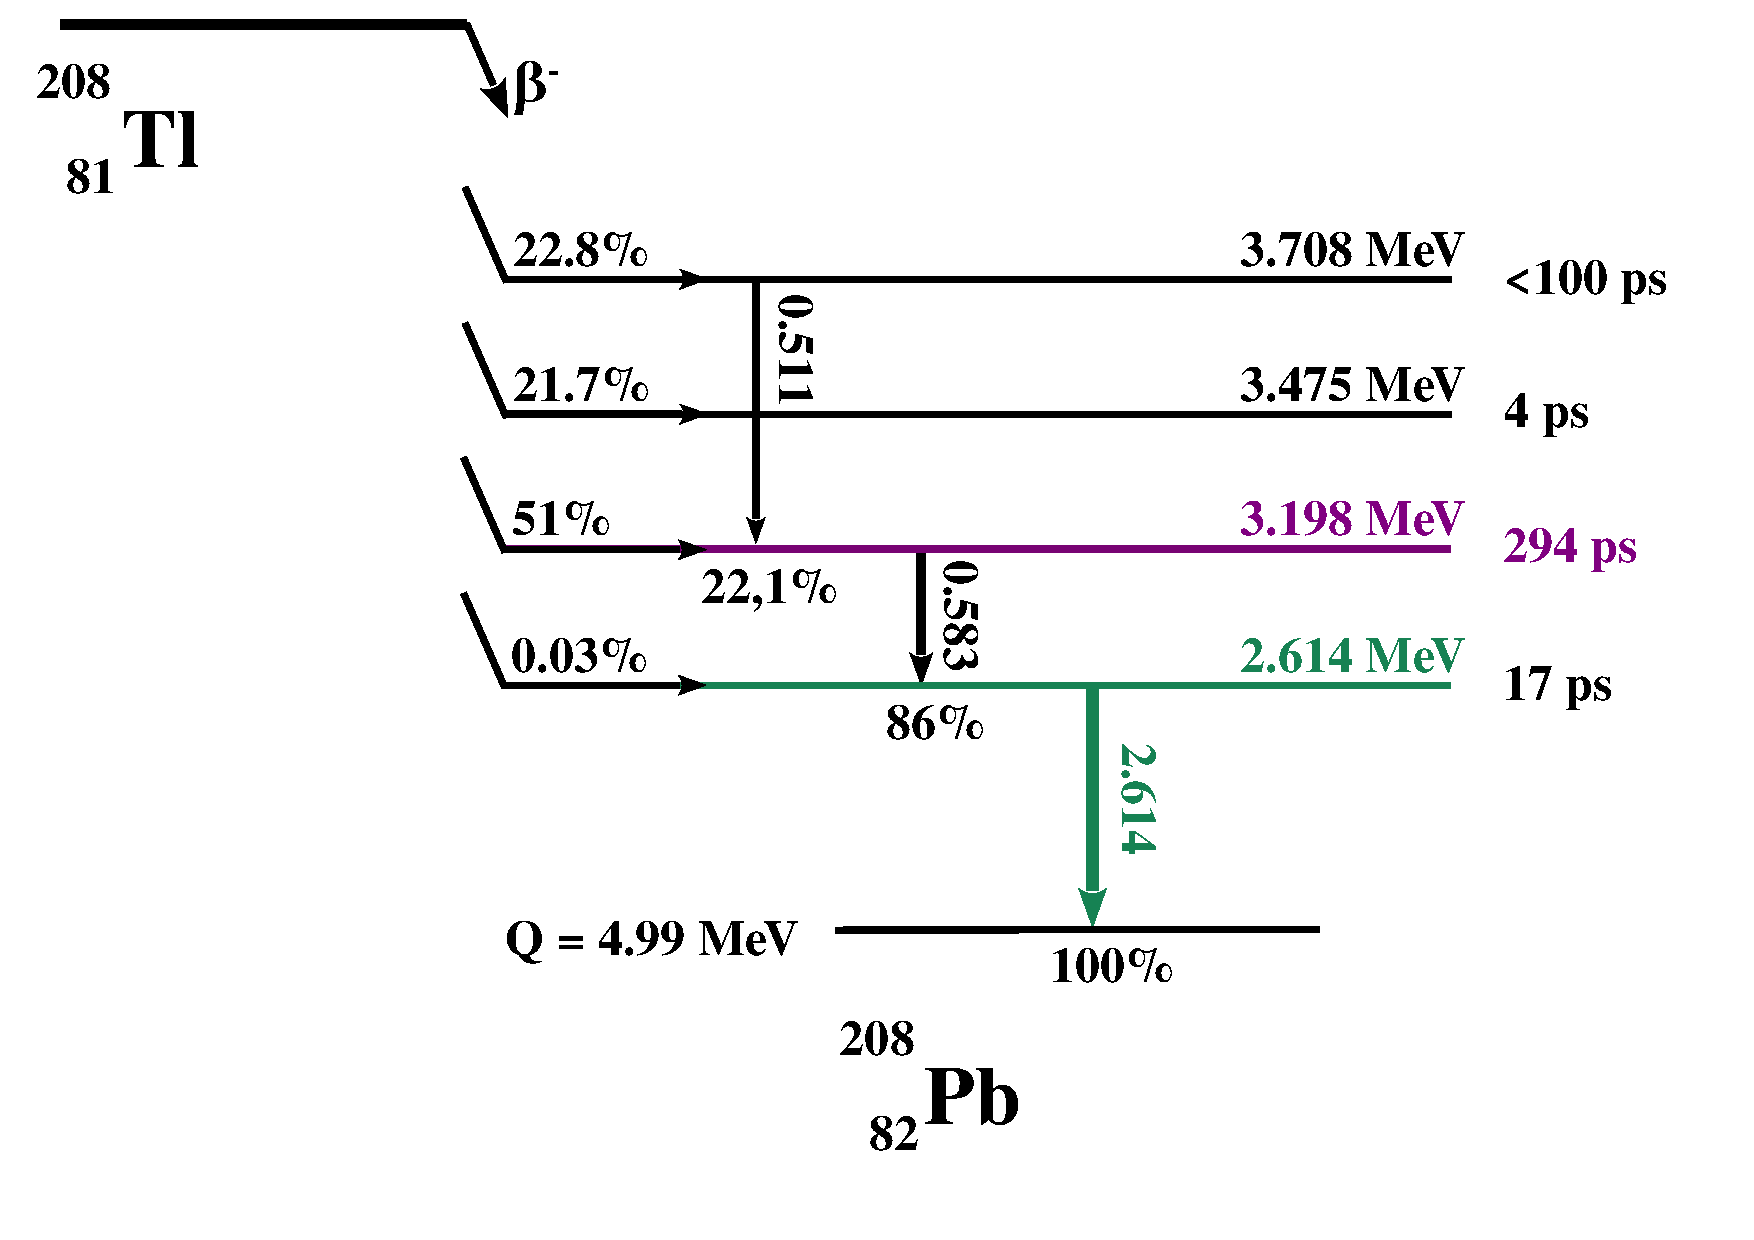
\includegraphics[width=13cm]{timedifference/fig_timediff/Tl_decay_scheme.pdf}
  \caption{Simplified desintegration scheme for \Tl\ isotope.
    The level in red has a significant life time of $294$ ps and can be useful in internal backgroung rejection.
  \label{fig:Tl_scheme}}
\end{figure}


For this study, we are focusing on the internal conversion process coming from the contamination of \Tl\ in the source foils.
Regarding the simplified desintegration scheme of the \Tl\ isotope (Fig.~\ref{fig:Tl_scheme}), we see that the $\beta$ desintegration has $51\%$ of probability to fall on the $294$ ps-life time exited level.
To decay to \Pb, the exited isotope has $100\%$ of probability to decay emmiting a $\gamma$ of $2.6$ keV.
In $0.2\%$ of cases, one of the orbital electron can interact with the exited nucleus and decay through internal conversion.
To summarise, decays where a \Tl\ nucleus emmits a $\beta$ particle and then an electron comming from internal conversion of the $2.6$ MeV-$\gamma$ represents $75\%$ of the total $\beta$ decays.
In this case, the internal conversion electron is time-delayed of $294$ ps compared with the $\beta$ particle.
We aim to use this delayed electron to discriminate \Tl\ internal background from signal and other internal backgrounds.





\begin{itemize}
\item trop de \Tl\ dans les sources par rapport aux spec
\item donc besoin d'une méthode de réjection spécifique pour \Tl\
\item pas gênant au niveau du démonstrateur (pour cela regarde le nombre d'événements de Tl208 attendus après l'optimisation des coupures avec le niveau de Tl208 mesuré par Bipo-3, je pense que c'est moins d'1 evt), mais cela peut être gênant pour une manip à 500 kg.y
\item avant de parler de la réjection avec le temps de vol, parler des autres réjections du Tl208 : bdf interne = 1 électron de conversion + 1 électron bêta -> l'électron de plus haute énergie a un pic en énergie (montrer une figure de simulation pour illustrer) et commenter avec le fait que la résolution en énergie s'améliore entre NEMO-3 et le démonstrateur. Donc normalement cette réjection sur l'énergie individuelle est plus efficace avec le démonstrateur.
\item Schema désintégration
\item Internal conversion -> reconnaître le Tl avec gamma $2.6$ MeV
\item Préciser l'énergie de l'électron de conversion associé (ou plutôt les énergies : raies K, L ...)
\item Un des deux gamma est retardé de 294 ps, puis conversion interne -> donner le proportion (nb d'ev attendus, dans la ROI)
\item Avant d'entrer dans le détail préciser le principe de la réjection par temps de vol.
L'électron de plus haute énergie est en retard, avec un retard en moyenne de 294 ps pour la plupart des niveaux (discuter un peu le schéma de désintégration, dans quel cas il sera en retard).
Ensuite dire que tu as quantifié le pourcentage d'électrons de haute énergie en retard avec une simulation "parfaite" i.e. avec une résolution en  temps  nulle.,
\end{itemize}

%% Internal conversion occurs after $\beta$ or $\alpha$ radioactive decays leaving the nucleus exited.
%% Then a $\gamma$ particle is emitted and transfers its energy to an atomic electron which results in ejection of this electron from the atom.
%% The emitted electron has an energy corresponding to the energy of previously exited nucleus reduced by the electron binding energy.
%% After the internal conversion, electrons reorganise.
%% The hole in internal layer is filled by an electron from an external layer (emitting an X ray).\\
%% The probability for an atomic electron to be ejected decreases with the initial binding energy.
%% Thus, electrons from K layers have a higher probability to be converted (see Fig.~\ref{fig:Tl_IC}).

\section{Describe mathematically internal events}

\subsection{The internal probability}
\begin{itemize}
\item outil déjà existant, déjà utilisé dans NEMO-$3$
\item identifier les ev venant de la source
\item détailler chaque terme
\item étudier l'influence du terme $\sigma_{l}$ dans la proba interne (on avait trouvé 0.03 ns pour avoir une Pint plate pour la 0nu)
\end{itemize}

\subsection{The exponential probability}
\begin{itemize}
\item besoin de décrire les ev conversion interne, avec une loi de probabilité
\item Avec un détecteur qui mesurerait parfaitement les temps et les énergies, la loi t(max) - t(min) serait une loi exponentielle, en pratique il faut la convoluer avec une gaussienne.
\item description de l'exponentially modified gaussian avec les paramètres des deux distrib (expo et gaus)
\item Ici montrer une distribution de Pexp pour des evts Tl208 (si possible aussi uniquement pour les evts Tl208 qui ont un Delta t(resolution parfaite) > 0
\item Decrire aussi comment on passe de la probabilité exponentielle modified gaussian à la probabilité cumulée, qui est celle sur laquelle tu vas couper.
\end{itemize}

\section{Event selection}
\begin{itemize}
\item cut Pint/Pexp
\item Montrer un biplot Pint/Pexp pour les evts Tl208 en représentant la coupure.
\item Optimisation of event selection: cut on delta t
\item 208Tl cut efficiency
\item cut efficiencies on 0nubb and other backgrounds
\item Donner le nb d'ev rejeté sur le nb d'ev total, puis sur le nb d'ev retardés
\end{itemize}

\section{Impact of \Tl\ rejection on the experiment's sensitivity}
Reprendre l'analyse de sensibilité faite avec Axel en rajoutant les cuts Pint/Pexp et delta t pour le final detector

\subsection{Influence of the calorimeter time resolution}
\begin{itemize}
\item Se servir des résultats de $\sigma_{t}$ trouvés au chap.~\ref{chap:Cobalt_study}
\item Mais dire que ces sigmas peuvent être améliorés
\item donc présenter l'évolution des résultats (efficacité de réjection et sensibilité) sur la réjection en fonction de la valeur de sigma t, à faire varier dans un certain range.
\item Tu pourrais avec une figure à 2D où tu montres l'efficacité relative 0nu (égale à 100\% avant cette coupure temporelle) en fonction de la réjection du Tl208 -> cela donne une courbe que tu parcoures et tu cherches à optimiser ton point de fonctionnement.
\end{itemize}


\section{Conclusions}




\begin{figure}
  \centering
  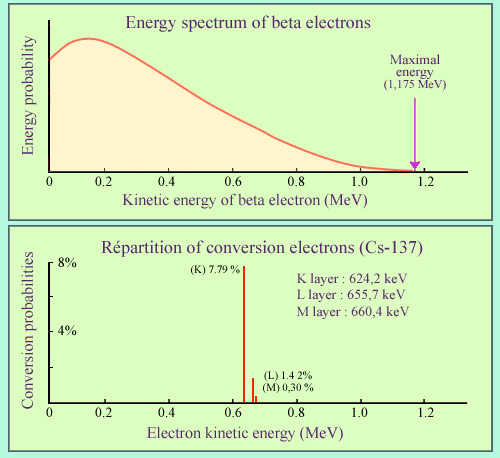
\includegraphics[width=9cm]{timedifference/fig_timediff/SpectreBeta_Cs137.jpg}
  \caption{\label{fig:Tl_IC}}

\end{figure}
